
%----------------------------------------------------------------------------------------
%	CHAP Seurat
%----------------------------------------------------------------------------------------

\chapterimage{blue-chapter-head_4-reduced.pdf} % Chapter heading image

\chapter{Seurat}\label{chap:Seurat}

\section{The Seurat language}

The Seurat language consists of statements that help with the analysis of
single cell RNA-sequencing data (scRNA-seq data). These statements cover a wide range of
functionality: loading scRNA-seq data, cleaning up the data, adjusting it (by normalization
or scaling), plotting it, computing extra information based on the data (principal components, markers,
etc.), aligning data from multiple samples, performing limma analysis on it and other
functionality.

Seurat statements can be typed in an Analysis script (see Chapter~\ref{chap:Analyses}).
The simplest way to see what Seurat statements are valid at a given line in an
analysis file, is to look at the suggestions offered by the context assistant. Figure~\ref{fig:ContextAssistantBeg}
and Figure~\ref{fig:ContextAssistantMid} show two examples of context assistants.
To activate the context assistant, just press
\keys{\return} in the script to generate an empty line. Placing the cursor on the empty line should
bring up the context assistant; in case you do not see it, press \keys{\space} on the empty line.
Moreover, to see all possible statements, you can use auto-completion like for all other
statements in a script (see Chapter~\ref{chap:Analyses}).

\begin{SCfigure}
  \centering
  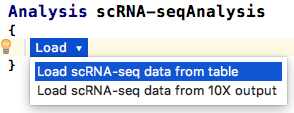
\includegraphics[width=\figWidthTiny]{figures/ContextAssistantBeg.png}
    \caption[Context assistant at beginning of script.]{\textbf{Context assistant at
    beginning of script.} At the beginning of the script, the
    context assistant suggests loading a Seurat object either directly from the output
    of the 10X, or from an expression table.}
\label{fig:ContextAssistantBeg}
\end{SCfigure}

\begin{figure}[h!tbp]
  \centering
  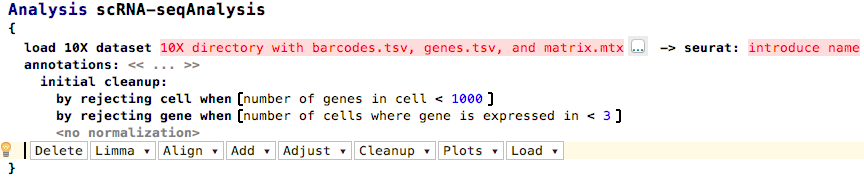
\includegraphics[width=\figWidthWide]{figures/ContextAssistantMid.png}
    \caption[Context assistant after loading one Seurat object.]{\textbf{Context
    assistant after loading one Seurat object.} Once we have Seurat objects
    available in the script, more Seurat statements become valid.}
\label{fig:ContextAssistantMid}
\end{figure}

To start writing analyses using Seurat, you need to import devkit
\texttt{org\allowbreak.campagne\allowbreak{}lab\allowbreak.metaR}
and language \texttt{org\allowbreak.campagne\allowbreak{}lab\allowbreak.metar\allowbreak.seurat}.
\noindent The following sections describe the kinds of statements offered by the MetaR
\texttt{org\allowbreak.campagne\allowbreak{}lab\allowbreak.metar\allowbreak.seurat} language.

\section{The Seurat object}
A Seurat object is a structure that stores scRNA-seq data and associated information. Many of
the Seurat statements result in the creation of a new Seurat object. Seurat objects and
references to these objects are represented with a purple foreground. Moreover, you can
study the associated information of a Seurat object in the inspector window, when clicking
on any such object or a reference to it. Figure~\ref{fig:PropertiesSeurat} shows the
information (properties) associated with a newly created Seurat object. These properties
are used by some statements to assess whether the input Seurat object is ready for the computations
required by the statement.

\begin{SCfigure}
  \centering
  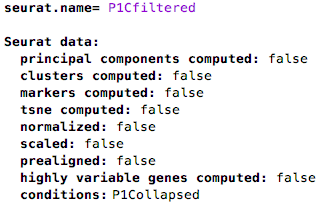
\includegraphics[width=\figWidthTiny]{figures/PropertiesSeurat.png}
    \caption[Properties view of a newly created Seurat object.]
    {\textbf{Properties view of a newly created Seurat object.} Many of the properties
    of this Seurat object are not yet computed. These properties are created automatically
    at the creation of the object.}
\label{fig:PropertiesSeurat}
\end{SCfigure}

\section{Loading Seurat objects}
There are two statements in the Seurat language for loading a Seurat object, one directly
from the files produced by 10X, and one from an expression matrix.

\subsection{Load 10X dataset}\label{subsec:Load10XDataset}
The \texttt{load 10X dataset} statement makes it possible to load a Seurat object directly
from the output files of 10X Genomics. The Seurat object and its properties become available
to the statements that follow the loading (until the line where it is deleted; see
Section~\ref{sec:OtherSeuratStatements}). You can create this statement by clicking
\menu{Load > Load scRNA-seq data from 10X output} in the context assistant, or by typing
the alias \texttt{load 10X dataset} on an empty line of Analysis (see Figure~\ref{fig:Load10XDataset})
for a new load 10X dataset statement).

\begin{figure}[h!tbp]
  \centering
  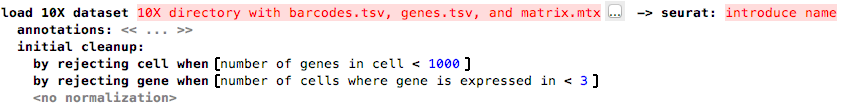
\includegraphics[width=\figWidthWide]{figures/Load10XDataset.png}
    \caption[New load 10X dataset statement.]{\textbf{New load 10X dataset statement.}
    Use this statement to load a Seurat object from the output of 10X Genomics.}
\label{fig:Load10XDataset}
\end{figure}

When creating a new \texttt{load 10X dataset} statement, the \texttt{by rejecting cell when}
strategy and \texttt{by rejecting gene when} come prefilled by default with certain upper
thresholds, but these strategies can be changed.

\paragraph{input directory} This field of \texttt{load 10X dataset} should point to
the directory produced by 10X Genomics that contains the following three files: ``barcodes.tsv",
``genes.tsv" and ``matrix.mtx". Unless the directory you specify exists on the disk and it contains
these three files, the input directory field will be shown on a red background. Notice that
this field has a button to let you select the directory.

\paragraph{annotations} The annotations are references to group usages (see
Section~\ref{sec:ColumnGroupUsage}). They allow you to attach more information to
the data loaded from 10X Genomics. For instance, if you load data that corresponds
to a certain patient and a certain state of the sample (condition),
you would annotate the Seurat object with a reference to a group usage that represents the
patient and with a reference to a group usage that represents the state (see
Figure~\ref{fig:ExampleLoad10XDataset}).
These annotations are used by the expression tables generated from the Seurat object
in the limma statements (see Section~\ref{sec:LimmaSeurat}). Note that you
need to create groups and group usages in a Column Group Container root node
in the model of your solution. If a Column Group Container does not exist in
the model, than you have to create one (see Section~\ref{sec:ColumnGroupContainer}).

\paragraph{cleanup strategies}
There are three possible strategies available when loading data from 10X Genomics: rejecting
a cell whose number of genes is lower or higher than a threshold, rejecting a
gene when the number of cells it appears in is greater or smaller than a threshold, and
normalizing the data at loading time. The cleanup strategies are explained in
Section~\ref{sec:CleanupSeurat}.

\paragraph{output} The output of the \texttt{load 10X dataset} statement is a Seurat object.
You need to set the name of this object.

\paragraph{Example} Figure~\ref{fig:ExampleLoad10XDataset} presents an example of a
\texttt{load 10X dataset} statement.

\begin{figure}[h!tbp]
  \centering
  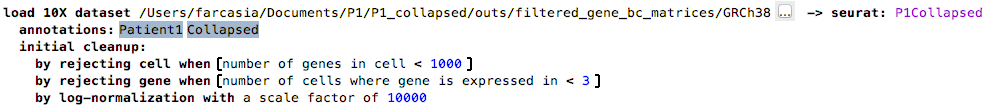
\includegraphics[width=\figWidthWide]{figures/ExampleLoad10XDataset.png}
    \caption[Example of load 10X dataset statement.]{\textbf{Example of load 10X dataset statement.}
    In this example, we load data for a patient denoted ``Patient1", from a sample of collapsed
    tubules tissue. As a result, we annotate this Seurat object with ``Patient1" and
    ``Collapsed". Furthermore, we reject the cells with less than 1000 genes expressed in
    them, and the genes that can only be found in less than 3 cells. Finally, we normalize
    the data using a scale factor of 10000.}
\label{fig:ExampleLoad10XDataset}
\end{figure}

\subsection{Load dataset from table}
The \texttt{load dataset from} statement makes it possible to load a Seurat object from a
table that contains expression data. You can create this statement by clicking
\menu{Load > Load scRNA-seq data from table} in the context assistant, or by typing
the alias \texttt{load dataset from table} on an empty line of Analysis. This statement
is identical in fields and behavior to the \texttt{load 10X dataset} statement, except
for the place of input (one is a directory generated by 10X Genomics, and one is a table).
Thus, we refer you to Subsection~\ref{subsec:Load10XDataset} for further details on the common fields.

\paragraph{input table}
The input table should have genes on the rows and cells on the columns.
Moreover, the table should have the row names. To reference a table
from this statement, you need to have a table available in the model (either by importing
it, or by obtaining it from other statements; see Section~\ref{chap:Tables}).

\paragraph{Example} Figure~\ref{fig:ExampleLoadTable} presents an example of a
\texttt{load data from table} statement.

\begin{figure}[h!tbp]
  \centering
  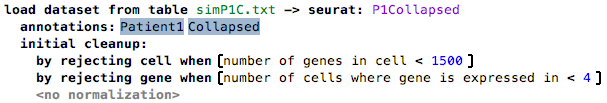
\includegraphics[width=\figWidthWide]{figures/ExampleLoadTable.png}
    \caption[Example of load data from table statement.]{\textbf{Example of load data from table statement.}
    In this example, we load data from a table with simulated data for a pacient
    denoted ``Patient1", and from a sample of collapsed tubules tissue.
    As a result, we annotate the Seurat object with ``Patient1" and
    ``Collapsed". Furthermore, we reject the cells with less than 1500 genes expressed in
    them, and the genes that can only be found in less than 4 cells. We do not normalize
    the data at loading time.} 
\label{fig:ExampleLoadTable}
\end{figure}

\section{Cleaning up Seurat objects}\label{sec:CleanupSeurat}
One important step in the analysis of scRNA-seq data is quality control on the data. In
Seurat, you can do that with the \texttt{cleanup seurat} statement. Usually, this
quality control step is done after observing some diagnostic plots on the data (
see Section~\ref{subsec:DiagnosticPlots} for diagnostic plots).

You can create this statement by clicking \menu{Cleanup} in the context assistant,
or by typing the alias \texttt{cleanup seurat} on an empty line of Analysis (see
Figure~\ref{fig:CleanupSeurat} for a new \texttt{cleanup seurat} statement). Note that in
the context assistant, you always need to specify a strategy that is going to be instantiated
in the \texttt{cleanup seurat} statement.

\begin{figure}[h!tbp]
  \centering
  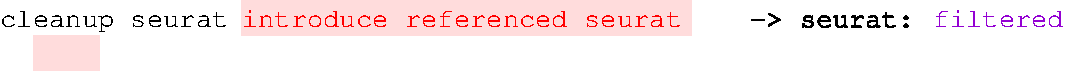
\includegraphics[width=\figWidthWide]{figures/CleanupSeurat.pdf}
    \caption[New cleanup seurat statement.]{\textbf{New cleanup seurat statement.}
    Use this statement to perform quality control on a Seurat object.}
\label{fig:CleanupSeurat}
\end{figure}

\paragraph{input Seurat} You need to specify the Seurat object on which quality control
is done. Only Seurat objects that are defined in previous statements are visible in the
current cleanup statement, due to scoping rules.

\paragraph{output Seurat} The statement creates a new Seurat object that represents the
input Seurat object with the modifications prescribed in the cleanup statement. The
\texttt{cleanup seurat} statement creates a default name for the output Seurat object,
but this name can be modified.

\paragraph{strategies} To introduce a strategy, you have to press \keys{\ctrl+\space}
in the red space on the second line of the statement. All the available strategies will
subsequently appear in the menu. In the next sections, we explain these strategies. Two
of these strategies are only available in the initial cleanup section of the loading
statements: the reject gene strategy and the normalization strategy.

\subsection{Reject gene strategy}
The \texttt{by rejecting gene when} strategy specifies a comparison operation where the
\texttt{number of cells where gene is expressed in} is compared to a threshold.
This strategy filters the input Seurat object by dropping the genes for which
the comparison is true. For this strategy, the left-hand side of the comparison can be
only \texttt{number of cells where gene is expressed in}.

\subsection{Reject cell strategy}
Another strategy is when you reject cells based on whether certain conditions are fulfilled.
Pressing \keys{\ctrl+\space} on the left-hand side of a condition in this strategy gives you
three possibilities: number of UMIs (unique molecular identifiers), number of genes and
percentage of mithocondrial genes in cell. This strategy filters the input Seurat object
by dropping the cells for which any of the comparisons is true. You can specify multiple
conditions in this strategy (see Figure~\ref{fig:ExampleCleanupSeurat} for an example).

\subsection{Regress out strategy}
Because single cell datasets often contain technical noise, batch effects, or even undesired
biological sources of variation, the cleanup statement offers a strategy to regress out
these sources of variation. You can write a list of such sources to be regressed out;
after introducing one element inside the square brackets of the regress out strategy, just
press \keys{\return} to introduce a new element (see Figure~\ref{fig:ExampleCleanupSeurat}
for an example). Note that this strategy also scales the data after regressing out the
variation, so it is adviced that it is the last strategy in the cleanup statement. As a result,
we obtain scaled data after the cleanup.

\subsection{Accept highly variable genes strategy}
It is common that you focus on the highly variable genes for downstream analysis; for this end,
you can use the \texttt{by accepting highly variable genes when} strategy. This will mark
the highly variable genes in the Seurat object. The highly variable genes are used by further Seurat
statements. To compute the higly variable genes, Seurat makes use of the average expression
and dispersion of each gene. The strategy allows you to set the cutoff for the average expression
and dispersion axis. The cutoff can be typed inside the square brackets of the strategy. To
introduce a new cutoff, just type \keys{\return} after the last one introduced, and press
\keys{\ctrl+\space} to see the available choices (see Figure~\ref{fig:ExampleCleanupSeurat}
for an example). Note that once you specify this strategy in the cleanup statement, an
output plot is pops up, that represents the dispersion versus average expression plot. You
need to provide a name for this plot.

\subsection{Normalization strategy}
Another strategy that can be used only in the cleanup section of the loading statements is the
normalization strategy. This strategy normalizes the data using the scale factor provided
in the strategy and log-transforms the result. There is also a separate statement for normalization (see
Subsection~\ref{fig:ExampleCleanupSeurat}).

\paragraph{Example} Figure~\ref{fig:ExampleCleanupSeurat} presents an example of a
\texttt{cleanup seurat} statement.

\begin{figure}[h!tbp]
  \centering
  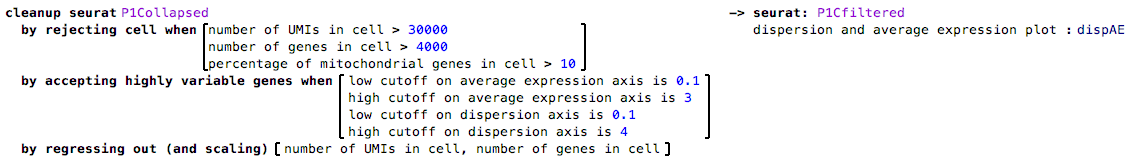
\includegraphics[width=\figWidthWide]{figures/ExampleCleanupSeurat.png}
    \caption[Example of cleanup seurat statement.]{\textbf{Example of cleanup seurat statement.}
    This illustrates almost all the features of the cleanup statement. We set a cutoff for
    all the axis, we reject cells based on three different conditions and we regress out
    unwanted variations for two different variables.}
\label{fig:ExampleCleanupSeurat}
\end{figure}

\section{Adjusting Seurat objects}
There are two statements in Seurat that are meant for standard adjusting
(pre-processing) the data: normalization and scaling. Some statements require that the
Seurat object is already normalized or scaled. For instance, the calculation of highly
variable genes needs a normalized Seurat object as input.

\subsection{Normalize Seurat object}
The normalization statement normalizes the expression data stored in the Seurat object and
log-transforms the result. You can create this statement by clicking
\menu{Adjust > Normalize} in the context assistant, or by typing
the alias \texttt{normalize seurat} on an empty line of Analysis (see Figure~\ref{fig:NormalizeSeurat}
for an example of a new \texttt{normalize seurat} statement).

\begin{figure}[h!tbp]
  \centering
  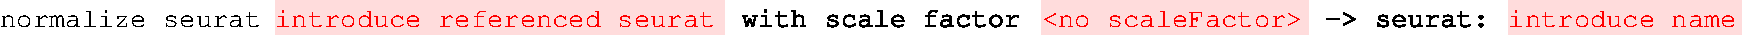
\includegraphics[width=\figWidthWide]{figures/NormalizeSeurat.pdf}
    \caption[New normalize seurat statement.]{\textbf{New normalize seurat statement.}
    A new \texttt{normalize seurat} statement with three fields to be completed.}
\label{fig:NormalizeSeurat}
\end{figure}

\paragraph{input Seurat}
The input Seurat object can be any Seurat object created in a previous statement, but it
should not be an already normalized Seurat object. You will receive an error if that is the
case.

\paragraph{scale factor}
You also need to specify the scaling factor for the normalization.

\paragraph{output Seurat}
The output is a normalized Seurat object. You need to introduce a name for
it.

\subsection{Scale Seurat object}
The scaling statement scales the data stored in the Seurat object.
You can create this statement by clicking \menu{Adjust > Scale} in the context assistant,
or by typing the alias \texttt{scale seurat} on an empty line of Analysis (see Figure~\ref{fig:ScaleSeurat}
for an example of a new \texttt{scale seurat} statement).

\begin{figure}[h!tbp]
  \centering
  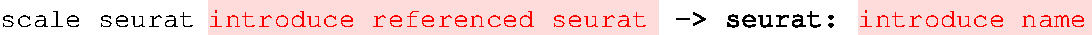
\includegraphics[width=\figWidthWide]{figures/ScaleSeurat.pdf}
    \caption[New scale seurat statement.]{\textbf{New scale seurat statement.}
    A new \texttt{scale seurat} statement with two fields to be completed.}
\label{fig:ScaleSeurat}
\end{figure}

\paragraph{input Seurat}
The input Seurat object can be any Seurat object created in a previous statement. Press
\keys{\ctrl+\space} to see the available choices.

\paragraph{output Seurat}
The output is a scaled Seurat object. You need to introduce a name for it.

\section{Plotting Seurat objects}
\subsection{Diagnostic plots}\label{subsec:DiagnosticPlots}
\subsection{Features plot}
\subsection{Features and total plot}

\section{Adding information to Seurat objects}
\subsection{Add principal component information}
\subsection{Add clusters information}
\subsection{Add markers information}

\section{Aligning Seurat objects}
\subsection{Pre-align Seurat objects}
\subsection{Align Seurat object}

\section{Limma for Seurat objects}\label{sec:LimmaSeurat}
\subsection{Pre-limma Seurat object}
\subsection{Limma voom}

\section{Other Seurat statements}\label{sec:OtherSeuratStatements}
\subsection{Merge Seurat objects}
\subsection{Delete Seurat object}
